\documentclass[11pt,a4paper,twoside,openright,titlepage]{report}

\usepackage[a4paper,top=3cm,bottom=3cm,left=3cm,right=3cm,marginparwidth=1.75cm]{geometry}

\usepackage[utf8]{inputenc}
\usepackage{amsmath}
\usepackage{amsthm}
\usepackage{amsfonts}
\usepackage{amssymb}
\usepackage{graphicx}
\usepackage{wrapfig}
\usepackage{bussproofs}
\usepackage{float}
\usepackage[italian]{babel}
\usepackage{fancyhdr}
\usepackage{verbatim}
\usepackage{afterpage}
\usepackage{contour}
\usepackage{bold-extra}
\usepackage[shortlabels]{enumitem}
\usepackage{listings}
\usepackage[center]{caption}
\usepackage{tabularx,ragged2e}
\usepackage{caption}

\newcolumntype{C}{>{\Centering\arraybackslash}X} % centered "X" column


\pagestyle{fancy}
\fancyhf{}
\fancyhead[LE,RO]{\thepage}
\fancyhead[RE]{ \nouppercase \leftmark}
\fancyhead[LO]{ \nouppercase \rightmark}

\graphicspath{ {./images/} }

\newcommand{\dt}{\Delta t} 
\newcommand{\dx}{\Delta x} 


\linespread{1.1}
\parindent 16pt

\title{Relazione IALab - Parte 3}
\author{Daniele Pautasso, Luca Sorrentino}
\date{} %hide date

\begin{document}

\maketitle

\chapter{Algoritmi di inferenza per reti Bayesiane}
In questo capitolo verranno trattati gli aspetti legati all'implementazione degli algoritmi di MPE e MAP, verranno analizzati i punti chiave dell’implementazione, partendo da aspetti di più basso livello (come la struttura dati scelta per rappresentare la cpt) a quelli di più alto livello (come la descrizione degli algoritmi stessi di MAP ed MPE).

\section{Implementazione}
L’implementazione è stata realizzata in python partendo completamente da zero, ovvero si è scelto di non usufruire della possibilità di avvalersi del codice fornito dalla repository ufficiale \texttt{aimacode}. Questa scelta ha portato ad un sostanzioso incremento del lavoro da svolgere coadiuvato però da una maggiore libertà espressiva e da una maggior consapevolezza delle operazioni effettuate.

\subsection{CPT}
La cpt richiede una struttura dati non banale per poter essere rappresentata. Tale elemento è formato da una lista di variabili associate, una lista di assegnamenti (la cui quantità dipende dai domini delle variabili associate) e un valore in corrispondenza ad ogni assegnamento. Sono stati provati diversi approcci per la rappresentazione di questi oggetti, cercando di trovare un equilibrio tra efficienza e comodità di accesso ai dati. Dopo alcune idee scartate (come liste di dizionari o matrici) si è optato per una lista di oggetti (Assignment) ognuno aventi come parametri: variabili, assignment e rispettivo valore. Questo metodo si è rivelato particolarmente comodo in quanto permette di avere sempre a disposizione tutte le informazioni necessarie e di poterle gestire in modo dinamico, al prezzo di una ridondanza del nome delle variabili associate, che viene ripetuto per ogni riga della cpt. Quando si è passati a lavorare su reti più grandi si è però subito palesato il limite di questo sistema di rappresentazione, ovvero l’ efficienza. Facendo un’analisi dei tempi di calcolo ci si è accorti infatti che la maggior parte del tempo veniva trascorsa nella routine di sum out.

\subsection{Implementazione del'operazione di  Sum Out}

\begin{minipage}{\linewidth}
	\centering
	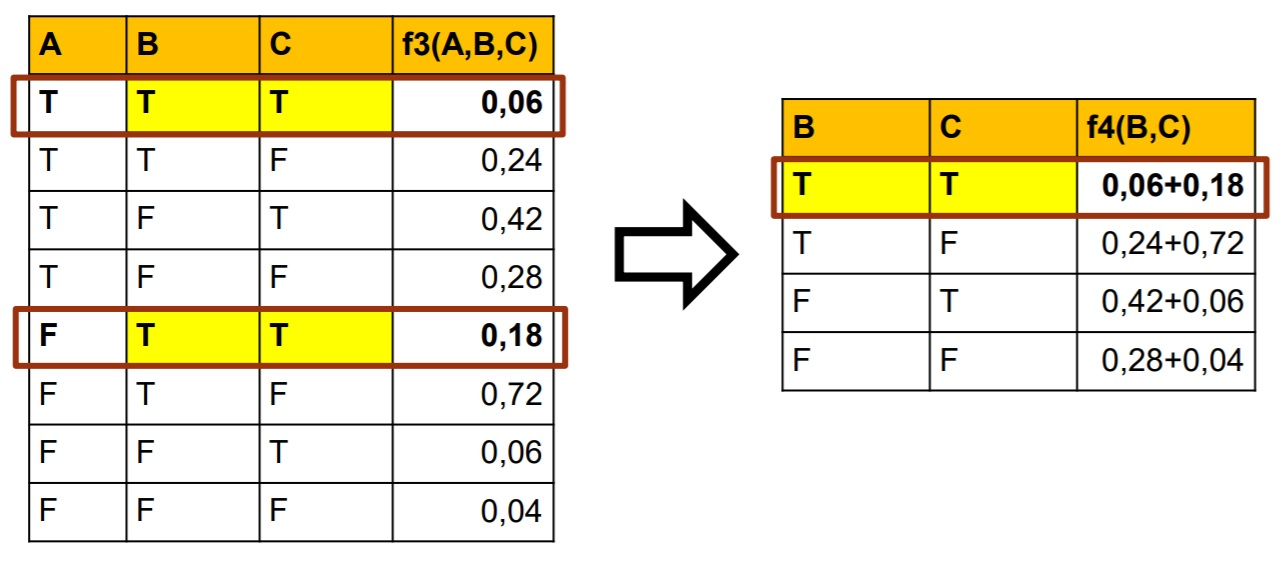
\includegraphics[width=0.9\linewidth]{map_teoria}
	\captionof{figure}{Esempio grafico del processo di Sum Out preso dalle slide a lezione.} 
	\label{map_teoria} 
\end{minipage}

Andiamo ora ad analizzare nel dettaglio questa procedura e ad individuare l’istruzione da ottimizzare per evitare il collo di bottiglia nel processore. L’operazione di sum-out consiste nella trasformazione di una cpt verso una seconda, il cui numero di colonne viene ridotto (e quindi anche di righe). Togliendo una colonna, molti degli assegnamenti che si differenziavano soltanto per il valore di tale colonna ora coincideranno (il numero di questi assegnamenti dipende dalla cardinalità del dominio della variabili eliminata). Di tutti gli assegnamenti ripetuti solo uno verrà assegnato alla nuova cpt e come valore associato a quell' assegnamento si utilizzarà la somma di tutti i valori associati agli assegnamenti ripetuti. Inizialmente questa operazione veniva eseguita ciclando su tutte le righe della cpt, per ogni riga si eliminava l’ assegnamento corrispondente a quello della variabile target e il risultato ottenuto lo si inseriva nella nuova cpt. Prima dell’inserimento però si doveva verificare che questo assegnamento non fosse già stato inserito in qualche passo precedente (questa operazione richiede di ispezionare tutta la nuova cpt). In base a questa verifica si decideva se creare una nuova riga con rispettivo valore o se limitarsi a sommare il nuovo valore con quello già inserito precedentemente in quella riga. Sebbene rimanga inevitabile ciclare per tutte le righe della cpt originaria, la medesima operazione non è necessaria per la cpt derivata. Ciò che effettivamente viene svolto  è una ricerca mediante una chiave, che può essere realizzata in tempo logaritmico se si usa una struttura a dizionario. Per cui si è scelto di modificare la struttura dati in un Oggetto avente come attributi una la lista (su cui sono segnate le variabili di associate a quella cpt, in modo da averle sempre disponibili ma senza ridondanze) e un dizionario del tipo: \texttt{cpt[tuple(assignment)] = value} (ovvero un dizionario in cui la chiave è data dagli assegnamenti delle variabili e il valore è dato  dalla cifra associata ad ogni assegnamento). Questo cambiamento ha snellito ulteriormente il codice permettendo di eliminare diverse funzioni ausiliarie e ha migliorato di molto i tempi di calcolo. A titolo esemplificativo lasciamo qui di seguito un estratto del codice sorgente dell’ operazione di sum out.

\begin{minipage}{\linewidth}
	\centering
	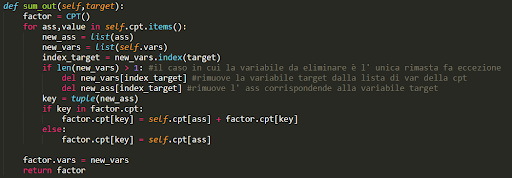
\includegraphics[width=0.9\linewidth]{codice}
	\captionof{figure}{Sorgente del metodo di Sum Out.} 
	\label{codice} 
\end{minipage}
 

\subsection{Altri metodi della classe CPT}
Gli altri metodi rilevanti della classe CPT sono:

\begin{itemize}
\item \textbf{Max Out}\\ 
Questo metodo è molto simile a quello di sum out se non per il valore associato agli assegnamenti che non è più calcolato mediante la somma dei due fattori ma che corrisponde al maggiore dei due.

\item \textbf{Pointwise Product}\\ 
Questo metodo combina due cpt andandone a creare una terza le cui variabili sono date dall’unione insiemistica delle variabili associate alle cpt di input. Per quanto riguarda il valore dei nuovi assignment prodotti, questo è dato dalla moltiplicazione dei dei valori degli assignemnt che sono stati combinati.

\item \textbf{Miglior assegnamento}\\
Questo metodo viene utilizzato nella retropropagazione degli assignment (che verrà spiegato più avanti nel paragrafo \ref{retropropagazione}). Data una lista di variabili (sottoinsieme di tutte le variabili della cpt) ed i rispettivi valori di assignment, restituisce il valore massimo tra tutti quelli associati agli assignments che combaciano con l'input ricevuto.
\end{itemize}
 
\subsection{Parser}
Avendo realizzato il software in python, non è stato possibile utilizzare il parser java fornito su moodle quindi si è deciso di svilupparne uno nostro adattandolo alle classi del nostro progetto. Durante parsificazione del file viene anche creato il grafo da cui estrarre l’ordine topologico, necessario poi per lo sviluppo degli algoritmi di MAP ed MPE.

\subsection{Grafo}
Questa classe costruisce il grafo che viene utilizzato per individuare l’ordine topologico dei nodi sulla rete. Tale struttura viene costruita e utilizzata solo durante la parsificazione del file e non influisce sui tempi di esecuzione dell’ algoritmo generale.
Ogni volta che si parsifica un nodo si trovano informazioni sui genitori di tale nodo. Nel dizionario rappresentante il grafo generale, invece di associare ogni nodo ai genitori, associamo ogni genitore ai rispettivi figli. In questo modo è possibile individuare facilmente quando un certo nodo è una foglia semplicemente verificando che non sia presente nel grafo (non è mai apparso tra i parent di qualche nodo). Per quanto riguarda i nodi root, questa caratteristica è facilmente inferibile dal file stesso. A questo punto abbiamo una lista di root da porre ad inizio dell’ ordine topologico e una lista di foglia da aggiungere in coda, restano da riordinare i nodi centrali. Dal momento che le reti bayesiani sono dei grafi e non degli alberi, sono possibili alcuni casi non banali da gestire, come ad esempio un collegamento diretto tra un nodo genitore, un nodo figlio e tra lo stesso nodo genitore ed il nodo figlio del suo nodo figlio. Questo tipo di problematiche ha reso impraticabili alcune implementazioni particolarmente vantaggiose dal punto di vista della complessità ma che non funzionavano su tutte le reti. L’algoritmo finale (che opera solo sulla lista non ordinata di nodi, da cui sono stati esclusi i nodi di root e quelli foglia) sposta i nodi nella lista ordinata solo se tutti i rispettivi parent sono già stati spostati, altrimenti passa ad analizzare il nodo successivo. Al termine della lista la ripercorre di nuovo da capo fino a che non sarà stato rimosso anche l’ultimo nodo. Nonostante scorra più volte la stessa lista non sono stati riscontrati particolari attese durante il parsing e il controllo sulla presenza dei parent assicura che il nodo verrà sempre inserito dopo di essi.

\subsection{Menu}
Si è deciso di gestire l’interazione con l’utente mediante un menu per agevolare la possibilità di settare comodamente più variabili senza dover ricompilare e per poter scegliere a tempo di esecuzione che tipo di operazione eseguire (es: map, mpe o benchmark).


\begin{minipage}{\linewidth}
	\centering
	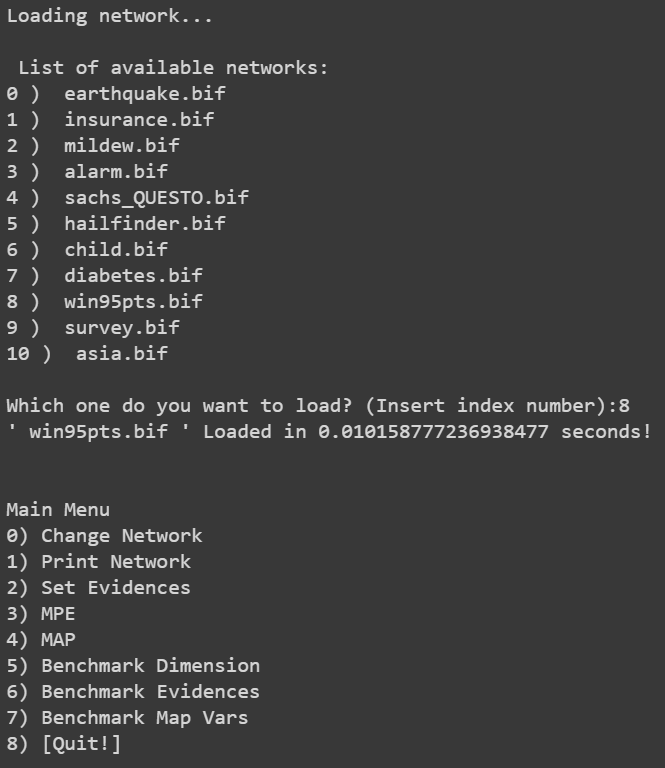
\includegraphics[width=0.5\linewidth]{menu}
	\captionof{figure}{Esempio di interazione con l' utente (si notino i tempi di attesa per il caricamente di win95pts, una rete di tipo "large").} 
	\label{codice} 
\end{minipage}

\section{Spiegazione MPE}
L’algoritmo di MPE segue un’impostazione molto vicina a quella proposta da Aimacode nel suo algoritmo di variable elimination. 
Sebbene siano state sperimentate più soluzioni per la gestione dei fattori prodotti durante l’esecuzione, alla fine si è optato per raccoglierli in una lista. Nel primo ciclo si percorre tutta la rete seguendo l’ordine topologico inverso e per ogni nodo se ne raccoglie la rispettiva cpt aggiungendola ad una lista. Durante questa operazione vengono rimosse tutte le entry contenenti assegnamenti in contraddizione con le evidenze fornite (se ce ne sono). Una volta aggiunto l’elemento si esegue un pointwise di tutti gli elementi attualmente presenti in lista che contengono la variabile associata al nodo target, e poi si esegue il max out sulla cpt risultate per eliminare tale variabile. Si prosegue quindi con una nuova lista avente il risultato appena ottenuto come unico elemento. Una volta completata la visita della rete si moltiplicano tutti gli elementi rimanenti nella lista e si calcola il valore massimo ottenuto in questa cpt finale. Questo valore verrà utilizzato per individuare il miglior assegnamento per tutti i nodi della rete. ( Spiegheremo in dettaglio questo metodo nel paragrafo \ref{retropropagazione}).

\section{Spiegazione MAP}
A differenza di MPE l’algoritmo richiede due cicli. Il primo ciclo è simile a quello visto in mpe ma oltre alla variabili di evidenza vengono ignorate anche quelle scelte come Map Var. Inoltre l’eliminazione dei fattori questa volta avviene con operazioni di sum out e non più max out. Il secondo ciclo avviene solo sulle restanti variabili map e consiste nella loro eliminazione tramite max out. Anche in questo caso si moltiplicano tutti i valori restanti nella lista per calcolare il valore totale da restituire e che verrà usato anche poi per il calcolo dei migliori assegnamenti dei nodi della rete.

\section{Retropropagazione dei migliori assegnamenti.}
Una volta individuato il valore finale (e quindi individuato il miglior assegnamento per l’ultimo nodo visitato) sarà possibile ripercorrere a ritroso la rete andando ad individuare i migliori assegnamenti per ogni nodo della rete. Per individuare tali valori si forniscono gli assegnamenti delle variabili padri (individuati dalla cpt dell’iterazione precedente) e si fissano tali valori facendo variare solo quello della variabile relativa al nodo, a quel punto si prende il valore massimo tra quelli disponibili. Si lascia qui di seguito un esempio per rendere più chiaro il procedimento.


\subsection{Esempio di Retropropagazione}\label{retropropagazione}
A titolo di esempio prendiamo la configurazione dell’esempio pubblicato su moodle. In quel caso otteniamo come valore risultante:

\lstset{language=Octave,basicstyle=\ttfamily}
\begin{lstlisting}[frame=single]
Rete Earthquake
Map Var: E,B,J,M
Best assignments
[0.9115897329]
\end{lstlisting}

Andando a esplorare in ordine topografico la rete, troviamo la cpt del primo noto (ovvero Burglary) con i valori aggiornati e troviamo facilmente la riga con l’assegnazione corretta

\lstset{language=Octave,basicstyle=\ttfamily}
\begin{lstlisting}[frame=single]
Current Node:  Burglary
Print CPT
['Burglary']
('True',)  ->  0.005803854
('False',)  ->  0.9115897329 -> max assignment
\end{lstlisting}

A questo punto passiamo all’iterazione successiva, tenendoci salvato il valore di (Burglary = False). Il nodo successivo è Earthquake.

\lstset{language=Octave,basicstyle=\ttfamily}
\begin{lstlisting}[frame=single]
Current Node:  Earthquake
Print CPT: 
['Earthquake', 'Burglary']
('True', 'True')  ->  0.0119705
('True', 'False')  ->  0.0135291 
('False', 'True')  ->  0.5803853999999999
('False', 'False')  ->  0.92079771 
\end{lstlisting}

A questo punto si procede isolando le righe in cui (Burglary = False) :

\lstset{language=Octave,basicstyle=\ttfamily}
\begin{lstlisting}[frame=single]
Current Node:  Earthquake
Print CPT: 
['Earthquake', 'Burglary']
('True', 'True')  ->  0.0119705
('True', 'False')  ->  0.0135291 -> candidate 
('False', 'True')  ->  0.5803853999999999
('False', 'False')  ->  0.92079771 -> candidate 
\end{lstlisting}

e se ne individua quella con valore massimo (0.92079771). Si aggiunga l’assegnamento di [Earthquake = False] alla lista e si proceda con le iterazioni successive. Andando ancora avanti si arriverà al nodo MaryCalls. Intuitivamente ci aspetteremmo di trovare Alarm ma essendo questa una variabili Non Map è stata eliminata dalla rete e i suoi figli sono diventati figli dei suoi parent. In sostanza il nodo MaryCalls ha come parent i parent di Alarm.

\lstset{language=Octave,basicstyle=\ttfamily}
\begin{lstlisting}[frame=single]
Current Node:  MaryCalls
Print CPT
['MaryCalls', 'Burglary', 'Earthquake']
('True', 'True', 'True')  ->  0.598525
('True', 'False', 'True')  ->  0.183055
('True', 'True', 'False')  ->  0.5922299999999999
('True', 'False', 'False')  ->  0.0095605 -> candidate 
('False', 'True', 'True')  ->  0.258975
('False', 'False', 'True')  ->  0.676455
('False', 'True', 'False')  ->  0.25677
('False', 'False', 'False')  ->  0.9395895 -> candidate 
\end{lstlisting}

Le informazioni su Burglary ed Earthquake sono esattamente quelle che abbiamo raccolto nelle iterazioni precedenti quindi possiamo continuare a reiterare il processo fino alla fine della visita arrivando alla conclusione:

\lstset{language=Octave,basicstyle=\ttfamily}
\begin{lstlisting}[frame=single]
Best assignments
[0.9115897329]

Burglary  ->  False
Earthquake  ->  False
MaryCalls  ->  False
JohnCalls  ->  False
\end{lstlisting}

\section{Verifica di correttezza delle implementazioni di MAP e MPE}
Una volta implementati gli algoritmi sono stati sperimentalmente verificati attraverso moltissime prove su varie configurazioni e su reti di diverse dimensioni. I risultati ottenuti sono stati confrontati con quelli forniti dall’ applicativo Samiam.






\section{Analisi delle performance}

Segue ora l’analisi dei risultati volta ad evidenziare le differenze principali tra il task di MPE e quello di MAP. Tale analisi verrà divisa in 4 punti, in ognuno dei quali si andrà ad analizzare un parametro diverso. 

\section{Reti Utilizzate}
I grafici sono stati ottenuti eseguendo i benchmark su 3 reti di diverse dimensioni e di diversi gradi di connettività per evidenziare al meglio come anche agendo su reti diverse tra loro, il risultato sia comunque costante. Queste reti sono state scaricate dalla repository url

Le reti su cui si è sperimentato sono:

\begin{itemize}
\item \textbf{Prima Rete}\\ 
Rete: Child
Num Nodi: 20
Average Markov Blanket size: 3.00

\item \textbf{Seconda Rete}\\ 
Rete: Alarm
N.nodi: 37
Average Markov Blanket size: 3.51

\item \textbf{Terza Rete}\\ 
Rete: Insurance
N.nodi: 27
Average Markov Blanket size: 5.19
\end{itemize}

\section{Analisi di dimensionalità}
Come variano le performance di MAP ed MPE al variare delle dimensioni della rete? Sebbene sia facile convincersi che una rete più grande avendo più nodi richieda più operazioni, meno facile è trovare un modo furbo per rendere tale evidenza.  Un’idea banale può essere quella di eseguire test su diverse reti di varie dimensioni, ma il numero di nodi non è l’unico fattore che influenza la complessità. La nostra proposta è stata quella di effettuare più test sulla stessa rete ma andando di volta in volta ad eliminare un nodo (partendo dai nodi foglia a salire). In questo modo il livello e il tipo di connessione dei nodi rimane costante, l’unica cosa che decresce linearmente è il numero dei nodi.

\begin{minipage}{\linewidth}
	\centering
	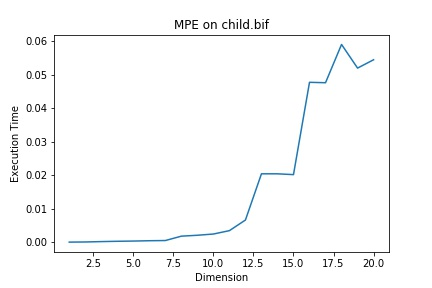
\includegraphics[width=0.9\linewidth]{dim_mpe_child}
	\label{dim_mpe_child} 
\end{minipage}

\begin{minipage}{\linewidth}
	\centering
	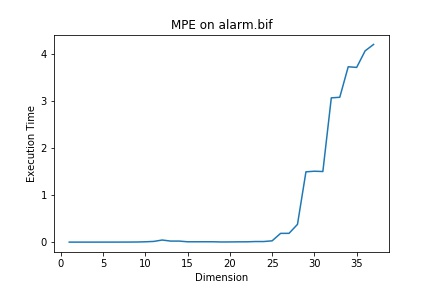
\includegraphics[width=0.9\linewidth]{dim_mpe_alarm}
	\label{dim_mpe_alarm} 
\end{minipage}
 
\begin{minipage}{\linewidth}
	\centering
	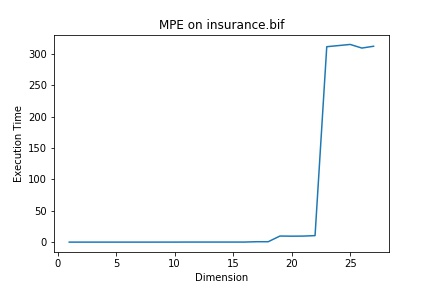
\includegraphics[width=0.9\linewidth]{dim_mpe_insurance}
	\label{dim_mpe_insurance} 
\end{minipage}

Come possiamo vedere dal grafico la complessità diminuisce mano a mano che la rete perde nodi. Come ci si potrebbe aspettare lo stesso avviene anche con il calcolo di MAP (nel caso di MAP si è scelto di selezionare di volta in volta, ed in modo casuale, un numero di variabili di MAP pari alla metà delle variabili totali rimaste). 

\begin{minipage}{\linewidth}
	\centering
	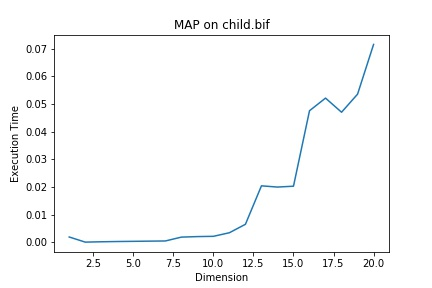
\includegraphics[width=0.9\linewidth]{dim_map_child}
	\label{dim_map_child} 
\end{minipage}

\begin{minipage}{\linewidth}
	\centering
	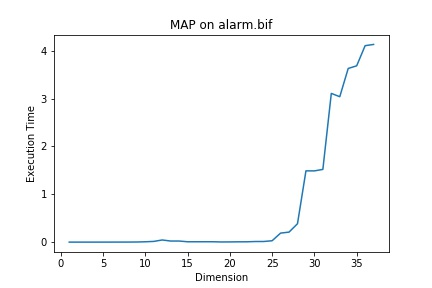
\includegraphics[width=0.9\linewidth]{dim_map_alarm}
	\label{dim_map_alarm} 
\end{minipage}
 
\begin{minipage}{\linewidth}
	\centering
	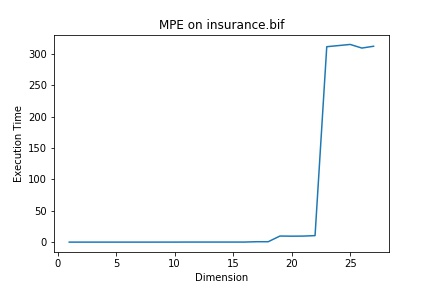
\includegraphics[width=0.9\linewidth]{dim_mpe_insurance}
	\label{dim_map_insurance} 
\end{minipage}


\section{Analisi della complessità}
Come variano le performance di MAP ed MPE al variare delle dimensioni della rete? (Dove per “complessità” si intende lontananza da un polytree). In questo caso non è stato possibile ricorrere ad un approccio completamente automatico ma ci siamo affidati ad un approccio euristico. Tra le descrizioni delle reti di esempio che ci sono state fornite vi è il campo “Average Markov Blanket Size”. Il Markov Blanket di un nodo è dato dal numero di genitori, figli e co-genitori. Questo valore indica il numero di nodi necessari affinché tale nodo risulti condizionalmente indipendente dai suoi vicini. Il valore fornito nella descrizione fornisce il livello medio generale di tutta la rete, per cui in questo contesto viene usato come stima del grado di connettività. Più questo valore è alto, più la rete è interconnessa e più è possibile trovare diversi percorsi che collegano due nodi (condizione da soddisfare per allontanarsi da un polytree). Nella scelta delle reti da usare come esempio, non è stato preso in considerazione solo il numero di nodi, ma anche questo parametro. Riprendendo i grafici appena proposti, possiamo notare che indipendentemente dal numero di nodi, il fattore di connettività maggiore sia dominante rispetto ai tempi di calcolo. Questo è reso particolarmente evidente dalla rete “Insurance” la quale, pur avendo quasi 10 nodi in meno rispetto ad alarm ha quasi due punti di AMbs in più, e infatti si può notare come i suoi tempi siano notevolmente maggiori rispetto a quelli di alarm. Da ciò se ne conclude che il numero di nodi ha un impatto sui tempi di calcolo ma questo valore dipende prevalentemente dal grado di connessione della rete (e questo vale per entrambi gli algoritmi).

\section{Analisi sul numero di variabili di evidenza}
Come variano le performance di MAP ed MPE al variare del numero di variabili di evidenza? Entrambi gli algoritmi cercano il miglior assegnamento possibile per un certo numero di variabili. Se questo numero diminuisce grazie al fatto che l’ assegnamento di alcune variabile viene già dato come input e non deve essere calcolato, è naturale pensare che l’ algoritmo necessiti di meno calcoli per arrivare alla soluzione.  L’algoritmo infatti non esegue l’ eliminazione di variabili di cui si ha già un’evidenza ed inoltre riduce tutte le cpt aventi assegnamenti incompatibili con tali evidenze (andando a ridurre notevolmente il carico di operazioni necessarie per il metodo di pointwise). Il costo complessivo è dominato dal fattore più grande che si viene a creare durante il processo, per cui limitare la grandezza della massima della cpt che si genera abbassa notevolmente i tempi di calcolo. Qui di seguito possiamo osservare dei casi di studio. 
L’andamento dei grafici conferma quanto ci si potrebbe aspettare, ovvero all’ aumentare delle evidenze il costo totale decresce.

\begin{minipage}{\linewidth}
	\centering
	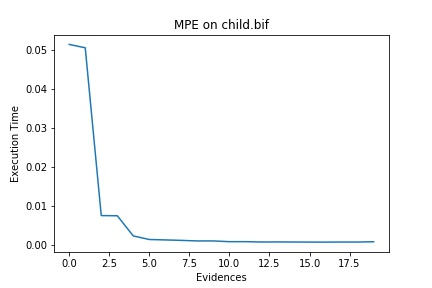
\includegraphics[width=0.9\linewidth]{evi_mpe_child}
	\label{evi_mpe_child} 
\end{minipage}

\begin{minipage}{\linewidth}
	\centering
	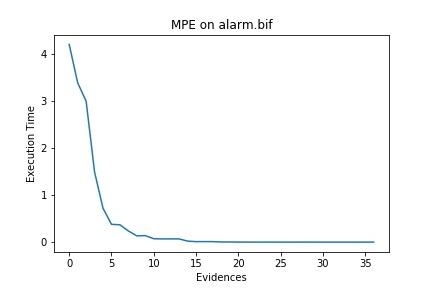
\includegraphics[width=0.9\linewidth]{evi_mpe_alarm}
	\label{evi_mpe_alarm} 
\end{minipage}
 
\begin{minipage}{\linewidth}
	\centering
	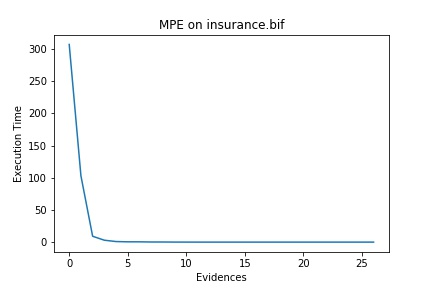
\includegraphics[width=0.9\linewidth]{evi_mpe_insurance}
	\label{evi_mpe_insurance} 
\end{minipage}

Il comportamento è lo stesso anche per MAP, in questo caso il numero di variabili di MAP selezionate corrisponde sempre alla metà di quelle totali.

\begin{minipage}{\linewidth}
	\centering
	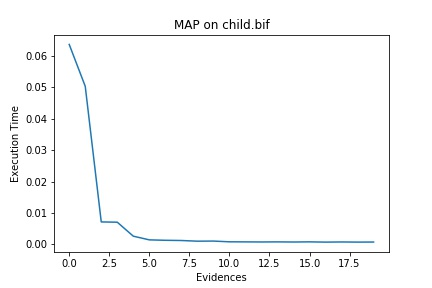
\includegraphics[width=0.9\linewidth]{evi_map_child}
	\label{evi_map_child} 
\end{minipage}

\begin{minipage}{\linewidth}
	\centering
	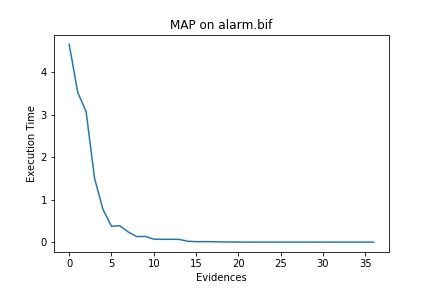
\includegraphics[width=0.9\linewidth]{evi_map_alarm}
	\label{evi_map_alarm} 
\end{minipage}
 
\begin{minipage}{\linewidth}
	\centering
	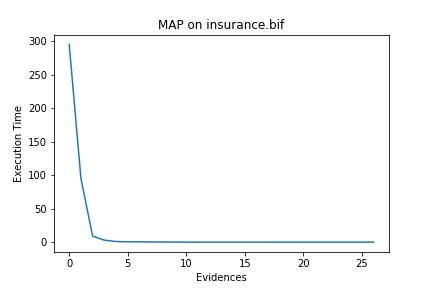
\includegraphics[width=0.9\linewidth]{evi_map_insurance}
	\label{evi_map_insurance} 
\end{minipage}


\section{Analisi sul numero di variabili di MAP}
Come variano le performance al variare del numero di variabili di MAP? Come abbiamo visto l’algoritmo di MAP esegue 2 visite della rete, la prima serve per eliminare le variabili che non sono state selezionate. Ora, dal momento che non vi sono grandi differenze tra operazioni di max out e sum out non ci si dovrebbero aspettare una crescita o decrescita lineare in base all’aumento di tali variabili. 

Lasciamo qui di seguito alcuni esperimenti effettuati su diverse reti con diverse configurazioni:

\begin{minipage}{\linewidth}
	\centering
	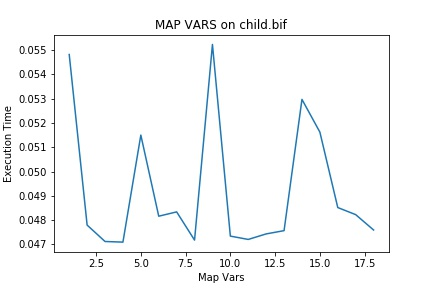
\includegraphics[width=0.9\linewidth]{map_child}
	\label{map_child} 
\end{minipage}

\begin{minipage}{\linewidth}
	\centering
	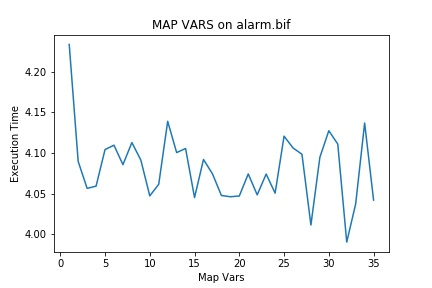
\includegraphics[width=0.9\linewidth]{map_alarm}
	\label{map_alarm} 
\end{minipage}
 
\begin{minipage}{\linewidth}
	\centering
	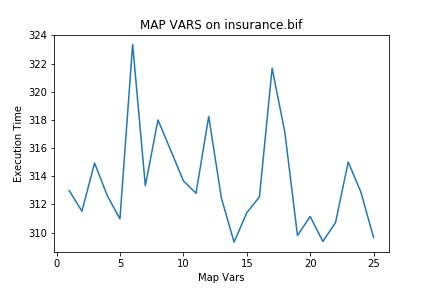
\includegraphics[width=0.9\linewidth]{map_insurance}
	\label{map_insurance} 
\end{minipage}

Ciò che si osserva è un’enorme variazione nei risultati ottenuti il che ci porta alla conclusione che le performance non sono tanto influenzate dal numero di variabili di MAP selezionate, ma dalla loro posizione all’interno della rete che influenza inevitabilmente l’ordine di eliminazione delle variabili. Infine si noti l’inefficienza di MAP rispetto al caso MPE (corrispondente alla parte finale del grafo, ovvero quella in cui vengono selezionate tutte le variabili come variabili di map). 



\chapter{Kalman Filters}

Il presente capitolo illustra alcuni esperimenti condotti sui Kalman filters e analizza i risultati ottenuti.

\section{Implementazione e librerie di supporto}
Come consigliato si è fatto uso della libreria Java EJML, la quale mette a disposizione una comoda rappresentazione delle matrici e delle relative operazioni. In particolar modo si è sfruttata la classe \texttt{SimpleMatrix} che permette di esprimere le operazioni tra matrici in modo astratto, facilitando di molto la lettura del codice a scapito di un'efficienza leggermente minore. È stata quindi implementata la classe \texttt{KalmanFilter}, utilizzata per eseguire tutti i test di seguito riportati.

\section{Simulazione di un processo}

Il processo scelto è lo spostamento un oggetto che si muove di moto uniformemente accelerato in due dimensioni (piano XY). Lo stato è quindi rappresentato dal vettore:

dove le componenti $x$ e $y$ rappresentano la posizione corrente dell'oggetto, mentre $v_x$ e $v_y$ rappresentano la velocità dello stesso.

La matrice di transizione di stato \textbf{A}, la matrice di control input \textbf{B} e il relativo vettore di control input \textbf{u} sono così definiti:

\begin{equation*}
\textbf{A} = 
\begin{bmatrix}
1 & 0 & \dt & 0 \\
0 & 1 & 0 & \dt \\
0 & 0 & 1 & 0 \\
0 & 0 & 0 & 1 \\
\end{bmatrix}
\qquad 
\textbf{B} = 
\begin{bmatrix}
\frac{1}{2}\dt^2 & 0\\
0 & \frac{1}{2}\dt^2\\
\dt & 0 \\
0 & \dt \\
\end{bmatrix}
\qquad 
\textbf{u} = 
\begin{bmatrix}
a_x \\
a_y \\
\end{bmatrix}
\end{equation*}
dove $\dt$ indica l'intervallo di tempo trascorso, idealmente, tra un'iterazione e la successiva (espresso in secondi). Poiché il modello di transizione di stato prevede che il prossimo stato (predetto) $\textbf{x}^{(p)}_{t+1}$ sia calcolato come $\textbf{x}^{(p)}_{t+1} = \textbf{Ax}+ \textbf{Bu}$, le entry delle  matrici sono tali da implementare le note leggi del moto uniformemente accelerato di seguito riportate:
\begin{equation*}
s' = s + v \dt + \frac{1}{2}a(\dt)^2  \qquad v' = v + a \dt
\end{equation*}
In particolare il vettore \textbf{u}, se assunto costante, permette di mantenere l'accelerazione invariata; tale assunzione può essere facilmente rilassata per modellare anche quei casi in cui l'accelerazione subisce delle variazioni note. In tutti i test condotti \textbf{u} è assunto costante ma l'accelerazione subisce comunque delle variazioni dovute al rumore di processo: essa è infatti soggetta a rumore che segue le distribuzioni gaussiane $\mathcal{N}(0; \sigma^2_{accX})$ e $\mathcal{N}(0; \sigma^2_{accY})$, rispettivamente per la componente x e y. Vista la particolare influenza che i cambiamenti di accelerazione hanno su posizione e velocità dell'oggetto, la matrice di covarianza del rumore di processo \textbf{Q} è definita come:
\begin{equation*}
\textbf{Q} = 
\begin{bmatrix}
(\frac{1}{2} \dt^2 \sigma_{accX})^2 & 0 & 0 & 0 \\
0 & (\frac{1}{2} \dt^2 \sigma_{accY})^2 & 0 & 0 \\
0 & 0 & (\dt \sigma_{accX})^2 & 0 \\
0 & 0 & 0 & (\dt \sigma_{accY})^2 \\
\end{bmatrix}
\end{equation*}
per semplicità si è utilizzata una matrice diagonale, assumendo che tutte le variabili di stato osservate siano tra loro indipendenti. Questo ovviamente non rispecchia fedelmente la realtà: posizione e velocità sono inevitabilmente legate tra di loro in quanto influenzate dalle stesse variazioni di accelerazione.

Le misurazioni si limitano invece alla sola posizione dell'oggetto: si simula pertanto una situazione in cui nessuna informazione relativa alla velocità viene resa disponibile al Kalman filter per mezzo di ipotetici sensori. 
Anche le misura di posizione è soggetta a rumore, che in questo caso segue le distribuzioni gaussiane $\mathcal{N}(0,\sigma^2_{posX})$ e $\mathcal{N}(0,\sigma^2_{posY})$; la relativa matrice di covarianza è definita di conseguenza come:
\begin{equation*}
\textbf{R} = 
\begin{bmatrix}
\sigma^2_{posX} & 0 \\
0 & \sigma^2_{posY} \\
\end{bmatrix}
\end{equation*}
Anche in questo caso si è utilizzata per semplicità una matrice diagonale, assumendo che le misurazioni dei sensori di posizione (e relativi errori) siano tra loro indipendenti.

È quindi possibile intervenire separatamente sulle deviazioni standard $\sigma_{accX}, \sigma_{accY}, \sigma_{posX}$ e $\sigma_{posY}$ per incrementare/diminuire a piacere il rumore cui sono soggetti il processo reale e le misurazioni ottenute dai sensori.

\subsection{Prestazioni al variare dell'errore}

Sono stati effettuati alcuni test variando sia il rumore di processo che quello di misurazione al fine di valutare le prestazioni del Kalman filter in diverse condizioni. Per semplicità in tutti i casi si è assunto $\sigma_{accX} = \sigma_{accY}$ e $\sigma_{posX} = \sigma_{posY}$;
nelle considerazioni che seguono si farà pertanto riferimento alle sole $\sigma_{acc}$ e $\sigma_{pos}$. Inoltre, lo stato iniziale reale e stimato non coincidono: si è infatti posto lo stato iniziale stimato $\mathbf{x_0} = \begin{bmatrix} 0 & 0 & 0 & 0 \end{bmatrix}^T$ e la relativa matrice di covarianza $\mathbf{P_0 = I}$, mentre lo stato reale è stato inizializzato come $\mathbf{x_{real}} = \begin{bmatrix} 5 & 20 & 3 & -3 \end{bmatrix}^T$. Infine, si è posto $\dt = 1$.

Se non diversamente specificato, in tutti grafici che seguono (per esigenze di rappresentazione) vengono riportati solo i dati relativi alla componente $x$ della posizione: valore reale, valore stimato e valore osservato.

\begin{itemize}
\item \textbf{Errore trascurabile}\\
In questo primo caso sono state poste $\sigma_{acc} = 0$ e $\sigma_{pos} = 10^{-5}$ per simulare una condizione in cui il processo reale segue fedelmente il modello e la misurazione dei sensori è pressoché perfetta. Si ricordi tuttavia che lo stato iniziale del Kalman filter e quello del processo reale non coincidono in questo primo scenario. Non è stato possibile predisporre un errore di misurazione nullo: infatti \textbf{P} tende rapidamente ad annullarsi e, se si assume anche \textbf{R} nulla, dopo poche iterazioni l'inversione della matrice $\mathbf{S = H P H^T + R}$  (operazione necessaria per il calcolo del Kalman Gain) fallisce in quanto la matrice risultante ha determinante nullo. 

Ad ogni modo, ponendosi nelle condizioni di errore trascurabile presentante inizialmente, dopo sole 4 iterazioni lo scarto tra variabili di stato reali e stimate risulta in media inferiore di $10^{-5}$. Inoltre la matrice \textbf{P} assume il seguente aspetto:
\begin{equation*}
\textbf{P} = 
\begin{bmatrix}
7 \times 10^{-9} & 0 & 3 \times 10^{-9} & 0 \\
0 & 7 \times 10^{-9} & 0 & 3 \times 10^{-9} \\
3 \times 10^{-9} & 0 & 2 \times 10^{-9} & 0 \\
0 & 3 \times 10^{-9} & 0 & 2 \times 10^{-9} \\
\end{bmatrix}
\end{equation*}
ovvero l'errore commesso nell'approssimare lo stato reale è praticamente nullo, come previsto. Si noti come emerge ugualmente una correlazione fra posizione e velocità per le componenti analoghe.

\item\textbf{Errore basso}\\
Per modellare una situazione più realistica si sono poste $\sigma_{acc} = 3$ e $\sigma_{pos} = 6$. In queste condizioni il Kalman filter approssima molto bene il processo, e recupera in fretta lo ``scarto" dovuto alle diverse condizioni iniziali.

\begin{minipage}{\linewidth}
	\centering
	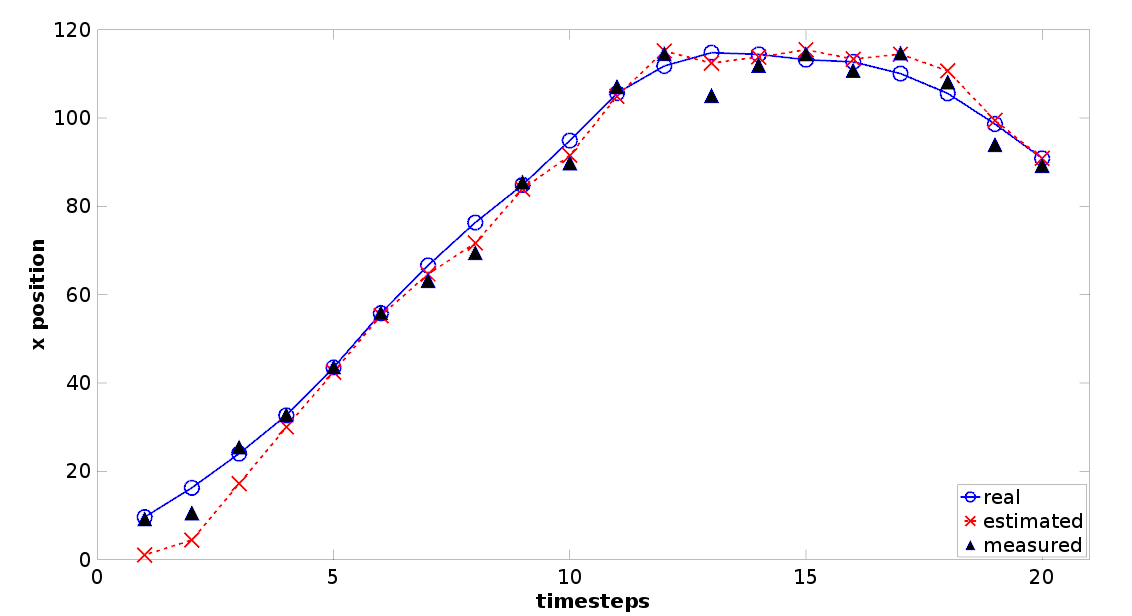
\includegraphics[width=\linewidth]{a3m6}
	\captionof{figure}{Stima nelle prime 20 iterazioni ponendo $\sigma_{acc} = 3$ e $\sigma_{pos} = 6$.}  
\end{minipage}

\item\textbf{Errore medio}\\
Si sono poste $\sigma_{acc} = 15$ e $\sigma_{pos} = 30$. In questo caso il rumore sembra influenzare maggiormente le prestazioni dello stimatore, come si evince dai due casi di seguito riportati. Il primo caso è da considerarsi ``fortunato" in quanto le misurazioni dei sensori seguono abbastanza fedelmente il processo reale; ciò consente al Kalman filter di fornire un'approssimazione tutto sommato buona. Nel secondo caso, invece, i valori osservati sono soggetti a delle oscillazioni più significative: queste hanno ripercussioni negative sulla stima.

\begin{minipage}{\linewidth}
	\centering
	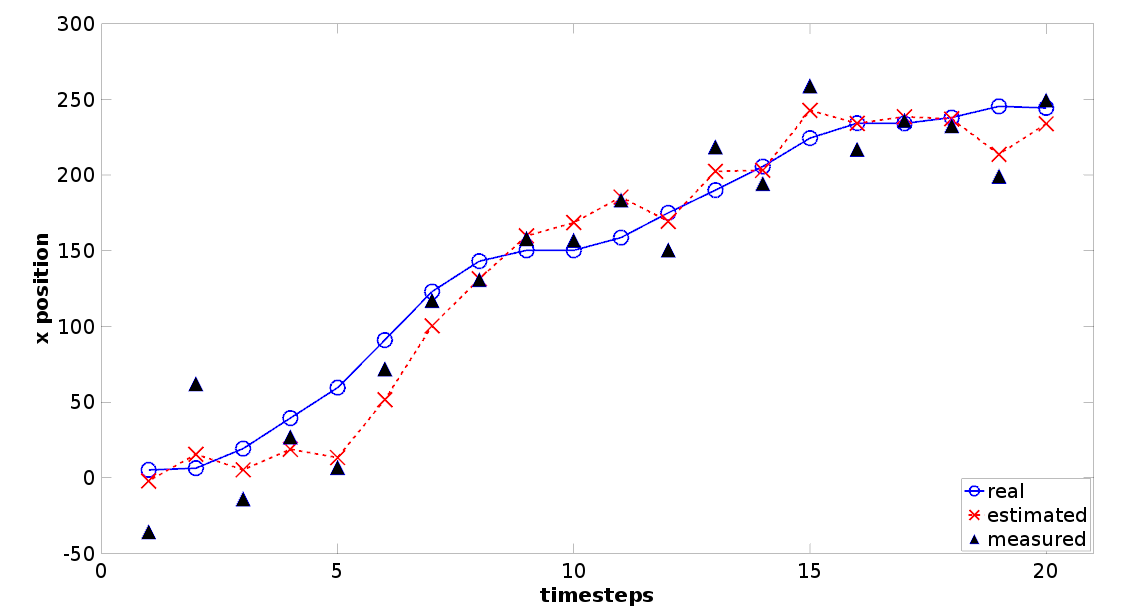
\includegraphics[width=\linewidth]{a15m30}
	\captionof{figure}{Stima nelle prime 20 iterazioni ponendo $\sigma_{acc} = 15$ e $\sigma_{pos} = 30$. Un caso ``fortunato" in cui le misurazioni non si discostano troppo dai valori reali.}  
\end{minipage}

\begin{minipage}{\linewidth}
	\centering
	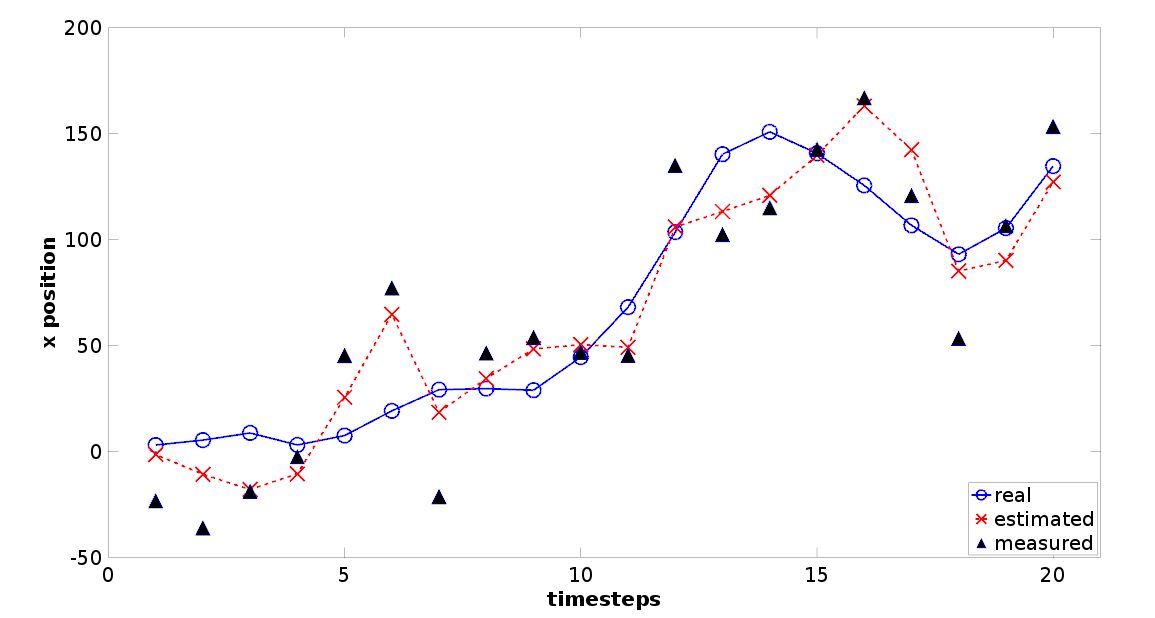
\includegraphics[width=\linewidth]{a15m30_2}	
	\captionof{figure}{Stima nelle prime 20 iterazioni ponendo $\sigma_{acc} = 15$ e $\sigma_{pos} = 30$. Un caso meno fortunato.}  
\end{minipage}

%\begin{center}
%\setlength\extrarowheight{2pt} % for a bit of visual "breathing space"
%\begin{tabularx}{0.8\textwidth}{|C|C|C|}
%\hline
%\textbf{Tolleranza componenti posizione} & \textbf{Tolleranza componenti velocità} & \textbf{Percentuale iterazioni entro le tolleranze}  \\\hline
%4 m & 4 m/s & $\sim$31\%\\
%\hline
%5 m & 5 m/s & $\sim$52\%\\
%\hline
%6 m & 6 m/s & $\sim$75\%\\
%\hline
%7 m & 7 m/s & $\sim$82\%\\
%\hline
%\end{tabularx}
%\end{center}

\newpage

\item\textbf{Errore elevato}\\
Infine, è stata trattata una situazione estrema ponendo $\sigma_{acc} = 50$ e $\sigma_{pos} = 100$. Si riportano di nuovo due diversi casi: in entrambi è possibile osservare come il Kalman filter non riesca a fornire consistentemente delle stime accurate a causa dell'elevata incertezza sia sul processo che sulle osservazioni. Durante alcune iterazioni il valore di posizione stimato e quello reale differiscono di quasi 200 metri, rendendo il tracking dell'oggetto molto difficoltoso.

\begin{minipage}{\linewidth}
	\centering
	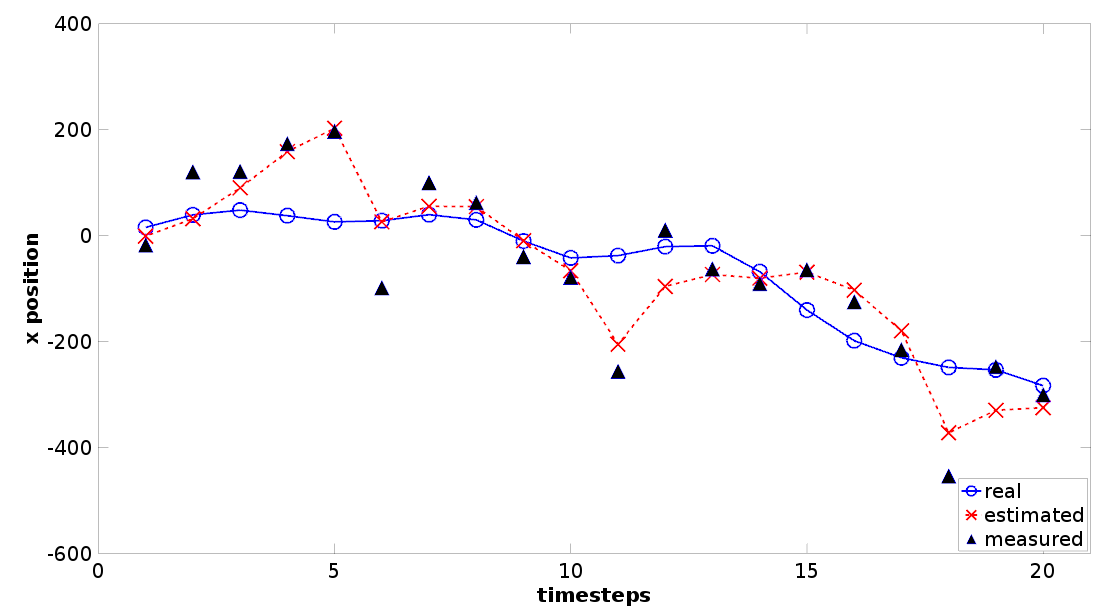
\includegraphics[width=\linewidth]{a50m100}
	\captionof{figure}{Stima nelle prime 20 iterazioni ponendo $\sigma_{acc} = 50$ e $\sigma_{pos} = 100$. Un primo caso.}  
\end{minipage}

\begin{minipage}{\linewidth}
	\centering
	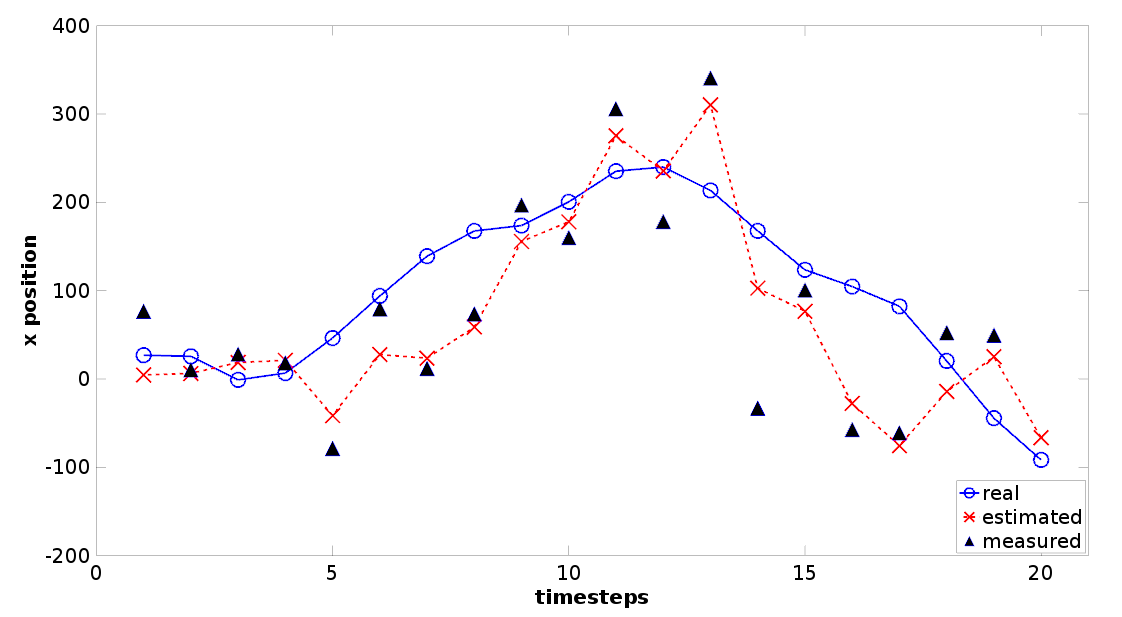
\includegraphics[width=\linewidth]{a50m100_2}
	\captionof{figure}{Stima nelle prime 20 iterazioni ponendo $\sigma_{acc} = 50$ e $\sigma_{pos} = 100$. Un secondo caso.}  
\end{minipage}

\newpage

\item \textbf{Errore di processo elevato ed errore di misurazione nullo}\\
Nel primo dei due casi si è posto $\sigma_{acc} = 100$ e $\sigma_{pos} = 0$. La matrice \textbf{P} si stabilizza già dopo le prime iterazioni, assumendo la forma:
\begin{equation*}
\small
\textbf{P} = 
\begin{bmatrix}
0 & 0 & 0 & 0 \\
0 & 0 & 0 & 0 \\
0 & 0 & 12071 & 0 \\
0 & 0 & 0 & 12071 \\
\end{bmatrix}
\end{equation*}
Tale risultato può essere intuitivamente giustificato come segue: poiché si ha la certezza che le misurazioni sono sempre perfettamente accurate, la varianza delle variabili di stato che rappresentano la posizione dell'oggetto è nulla; al contrario, poiché l'accelerazione è soggetta ad un rumore significativo, la varianza della velocità (e quindi l'incertezza sul suo valore reale) assume valori estremamente elevati. In figura \ref{velocity} sono riportati i dati relativi alla stima della velocità (componente x) in due differenti casi, che come previsto è piuttosto inaccurata a causa del rumore di processo.

\begin{minipage}{\linewidth}
	\centering
	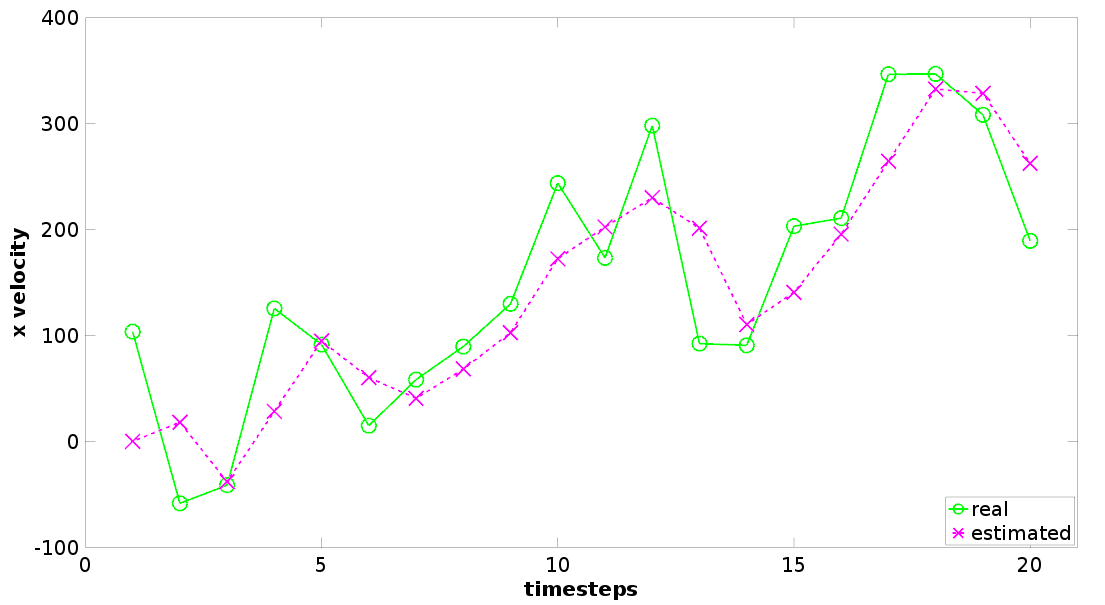
\includegraphics[width=\linewidth]{velocity}
	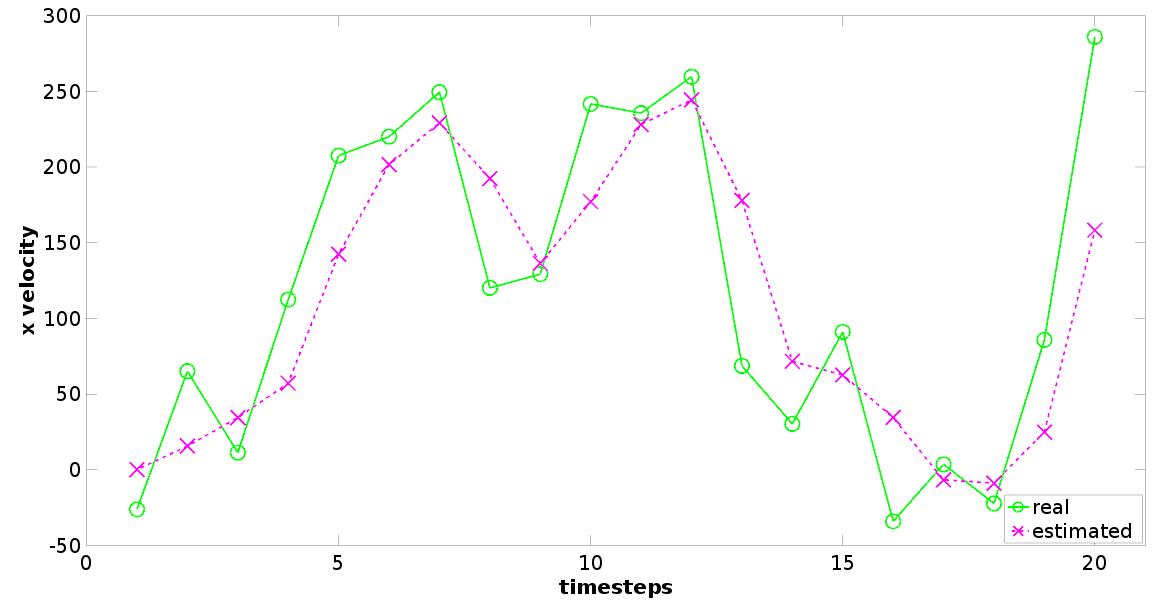
\includegraphics[width=\linewidth]{velocity2}
	\captionof{figure}{Stima nelle prime 20 iterazioni ponendo $\sigma_{acc} = 50$ e $\sigma_{pos} = 100$.}  
	\label{velocity}
\end{minipage}

\newpage

\item \textbf{Errore di processo nullo ed errore di misurazione elevato}\\
Simmetricamente, il secondo caso prevede $\sigma_{acc} = 0$ e $\sigma_{pos} = 100$. Le prime 20 iterazioni mostrano un andamento piuttosto stabile, come si evince dalla figura \ref{a0m100}.

\begin{minipage}{\linewidth}
	\centering
	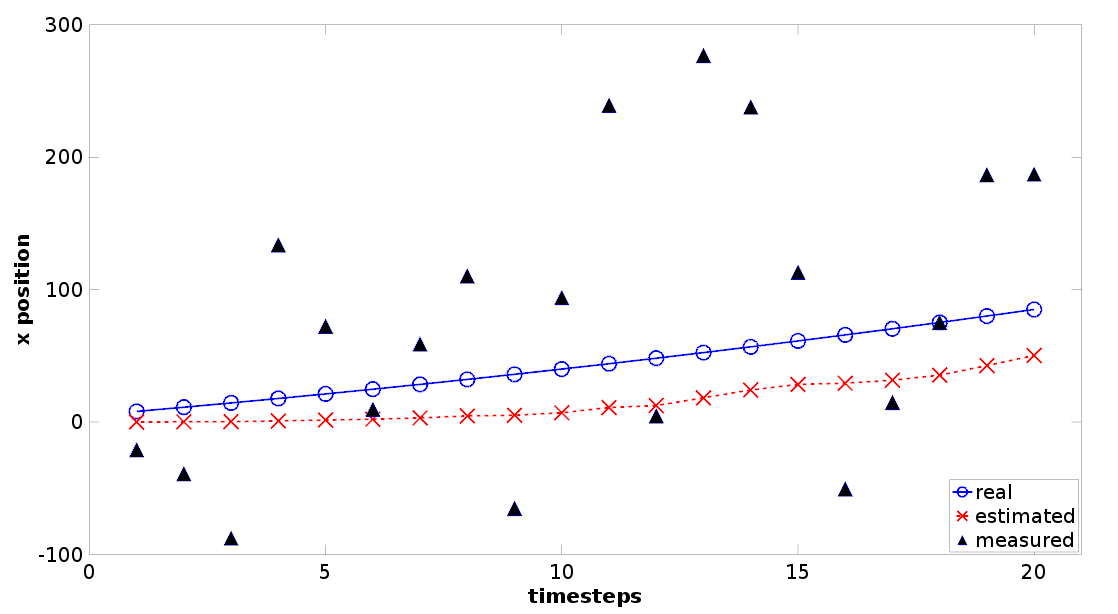
\includegraphics[width=\linewidth]{a0m100}
	\captionof{figure}{Stima nelle prime 20 iterazioni ponendo $\sigma_{acc} = 0$ e $\sigma_{pos} = 100$.}  
	\label{a0m100}
\end{minipage}

Pertanto, si è deciso di effettuare un numero maggiore di iterazioni per indagare il comportamento del Kalman filter sul lungo periodo. Dopo rispettivamente 500, 2500 e 5000 iterazioni la matrice \textbf{P} assume le seguenti forme: 

\begin{equation*}
\small
\textbf{P}_{500}= 
\begin{bmatrix}
60 & 0 & 1.2 & 0 \\
0 & 60 & 0 & 1.2 \\
1.2 & 0 & 0.0002 & 0 \\
0 & 1.2 & 0 &  0.0002 \\
\end{bmatrix}
\;
\textbf{P}_{2500} = 
\begin{bmatrix}
12.2 & 0 & 0.005 & 0 \\
0 & 12.2 & 0 & 0.005 \\
0.005 & 0 & 2.2 \times 10^{-6} & 0 \\
0 & 0.005 & 0 &  2.2\times 10^{-6} \\
\end{bmatrix}
\end{equation*}
\begin{equation*}
\small
\textbf{P}_{5000} = 
\begin{bmatrix}
6.2 & 0 & 0.001 & 0 \\
0 & 6.2 & 0 & 0.001 \\
0.001 & 0 & 3.2\times 10^{-7} & 0 \\
0 & 0.001 & 0 &  3.2\times 10^{-7} \\
\end{bmatrix}
\end{equation*}

La giustificazione di questo risultato è meno intuitiva. La spiegazione che è sembrata più verosimile è la seguente: si sa per certo che il processo viene simulato alla perfezione; infatti, il fenomeno reale non è affetto da alcun tipo di rumore e pertanto si comporta esattamente come previsto dal modello. Tuttavia, il Kalman filter non ha informazioni riguardo allo stato iniziale del processo reale, né può ricavarlo con assoluta sicurezza dalle misurazioni in quanto molto rumorose: per questo motivo vi è sempre un minimo di incertezza nella stima dello stato corrente (che tende a diminuire con l'aumentare delle misurazioni effettuate). Tale incertezza riguarda solo la posizione (poiché non si  hanno certezze riguardo al punto di partenza) e non la velocità, che viene stimata praticamente senza errori grazie al modello.
\end{itemize}

\subsection{Prestazioni al variare delle condizioni iniziali}
\label{known_state_subsec}

Alcuni dei test presentati nella sezione precedente sono stati ripetuti variando le condizioni iniziali, al fine di comprendere come queste influenzino la stima durante le iterazioni successive. Sono stati predisposti due scenari; in entrambi i casi il Kalman filter parte dallo stato iniziale $\mathbf{x_0} = \begin{bmatrix} 0 & 0 & 0 & 0 \end{bmatrix}^T$. Nel primo caso il processo reale parte dal medesimo stato (partenza perfetta), mentre nel secondo si impone arbitrariamente $\mathbf{x_{real}} = \begin{bmatrix} 220 & -137 & 17 & 28 \end{bmatrix}^T$ (partenza falsata). In caso di partenza perfetta si è posta $\mathbf{P_0 = 0}$ così che l'incertezza sullo stato stimato iniziale sia nulla.

\begin{itemize}
\item \textbf{Errore basso}\\
Sono state riprese le condizioni del primo test della sezione precedente, ponendo $\sigma_{acc} = 3$ e $\sigma_{pos} = 6$.
I risultati sono riassunti dai grafici nella figura \ref{ws_a3m6}. È possibile notare come nel caso con partenza perfetta il Kalman filter approssimi decisamente bene il processo, facilitato anche dal basso rumore. Nel caso con partenza falsata, invece, il divario tra posizione stimata e reale viene colmato in poche iterazioni.

\begin{minipage}{\linewidth}
	\centering
	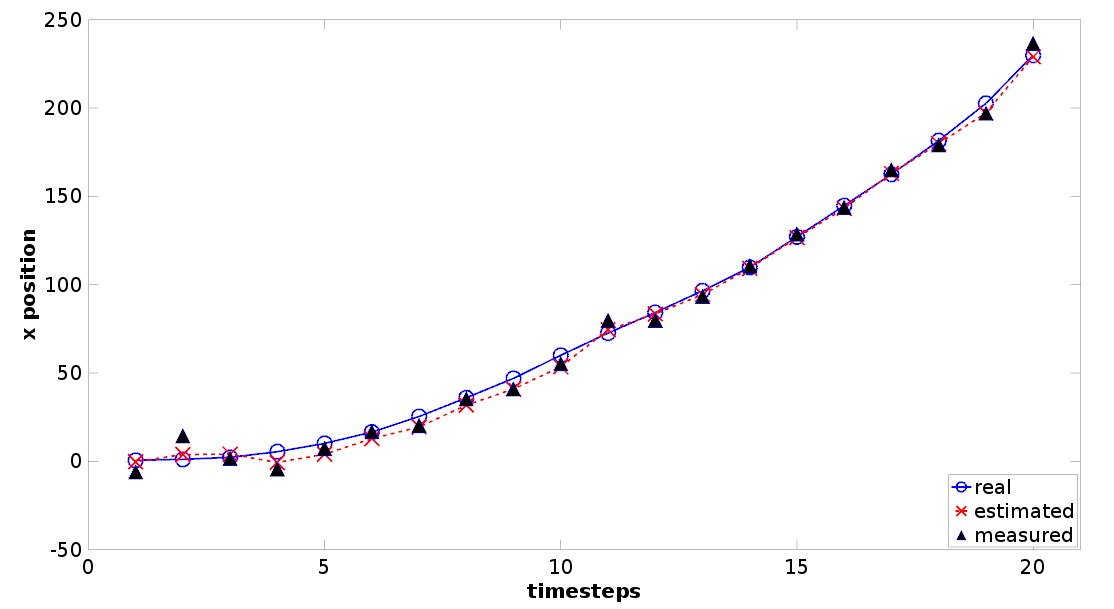
\includegraphics[width=0.9\linewidth]{ps_a3m6}
	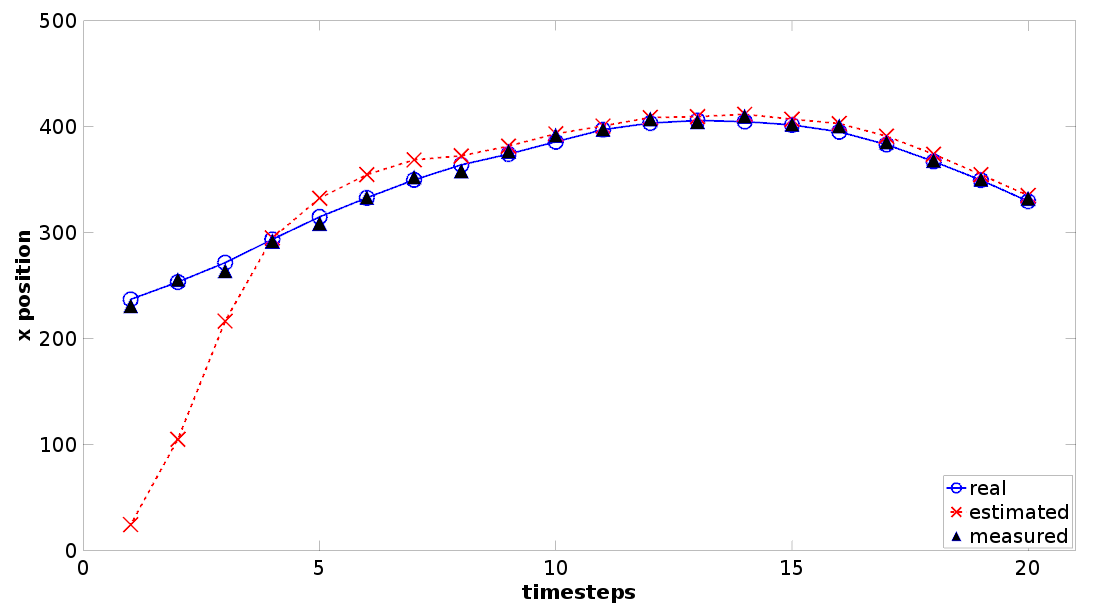
\includegraphics[width=0.9\linewidth]{ws_a3m6}
	\captionof{figure}{Stima nelle prime 20 iterazioni ponendo $\sigma_{acc} = 3$ e $\sigma_{pos} = 6$ (rispettivamente con partenza perfetta e falsata).} 
	\label{ws_a3m6} 
\end{minipage}

\item \textbf{Errore elevato}\\
Ponendo $\sigma_{acc} = 50$ e $\sigma_{pos} = 100$, anche una partenza perfetta non è sufficiente per mantenere l'approssimazione vicina al processo reale: dopo le prime iterazioni il Kalman filter viene deviato dalle osservazioni estremamente rumorose (figura \ref{ps_a50m100}). Sorprendentemente, lo stimatore è comunque in grado di approssimare (perlomeno a grandi linee) l'andamento generale del processo reale anche in queste situazioni estreme; ciò è vero soprattutto quando una serie di misurazioni si rivelano piuttosto precise, come accade nel caso illustrato in figura \ref{ws_a50m100} (decima iterazione e successive).

\begin{minipage}{\linewidth}
	\centering
	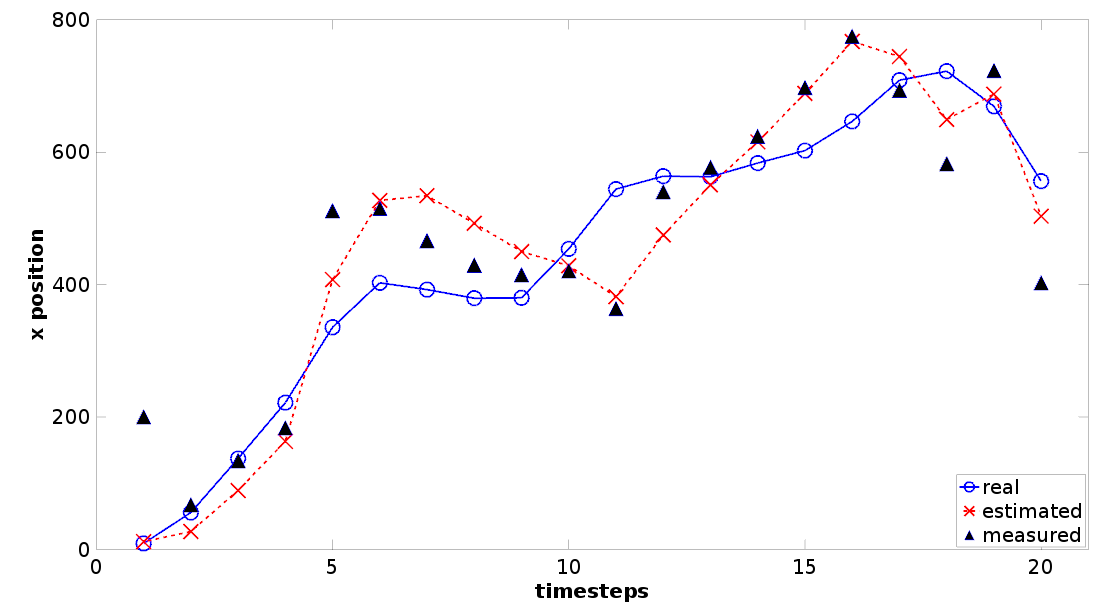
\includegraphics[width=\linewidth]{ps_a50m100}
	\captionof{figure}{Stima nelle prime 20 iterazioni ponendo $\sigma_{acc} = 50$ e $\sigma_{pos} = 100$ (partenza perfetta).}  
	\label{ps_a50m100}
\end{minipage}

\begin{minipage}{\linewidth}
	\centering
	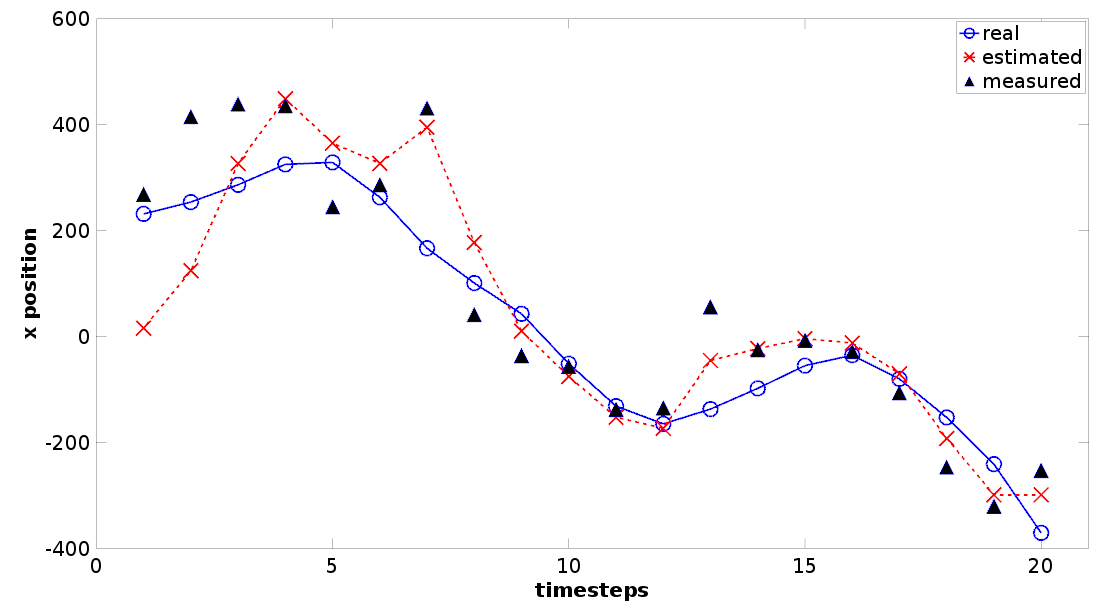
\includegraphics[width=\linewidth]{ws_a50m100}
	\captionof{figure}{Stima nelle prime 20 iterazioni ponendo $\sigma_{acc} = 50$ e $\sigma_{pos} = 100$ (partenza falsata).}  
	\label{ws_a50m100}
\end{minipage}

\newpage

\item \textbf{Errore di processo nullo ed errore di misurazione elevato}\\
In precedenza si è osservato come, nel caso in cui si pongano  $\sigma_{acc} = 0$ e $\sigma_{pos} = 100$, lo stimatore tenda a favorire il modello nella predizione dello stato successivo, in quanto esente da rumore. Questo fa sì che lo stato iniziale ricopra un ruolo importante: con una partenza perfetta il Kalman filter è in grado di simulare esattamente il processo reale, come testimonia la figura \ref{ps_a0m100}. Anche nel caso in cui lo stato iniziale stimato e quello reale non coincidano l'errore tende lentamente a diminuire con il passare delle iterazioni (figura \ref{ws_a0m100_long}): per quanto falsata possa essere la partenza, sul lungo periodo l'aumentare del numero di evidenze disponibili fa sì che il Kalman filter alteri la propria traiettoria, allineandosi progressivamente al processo reale.

\begin{minipage}{\linewidth}
	\centering
	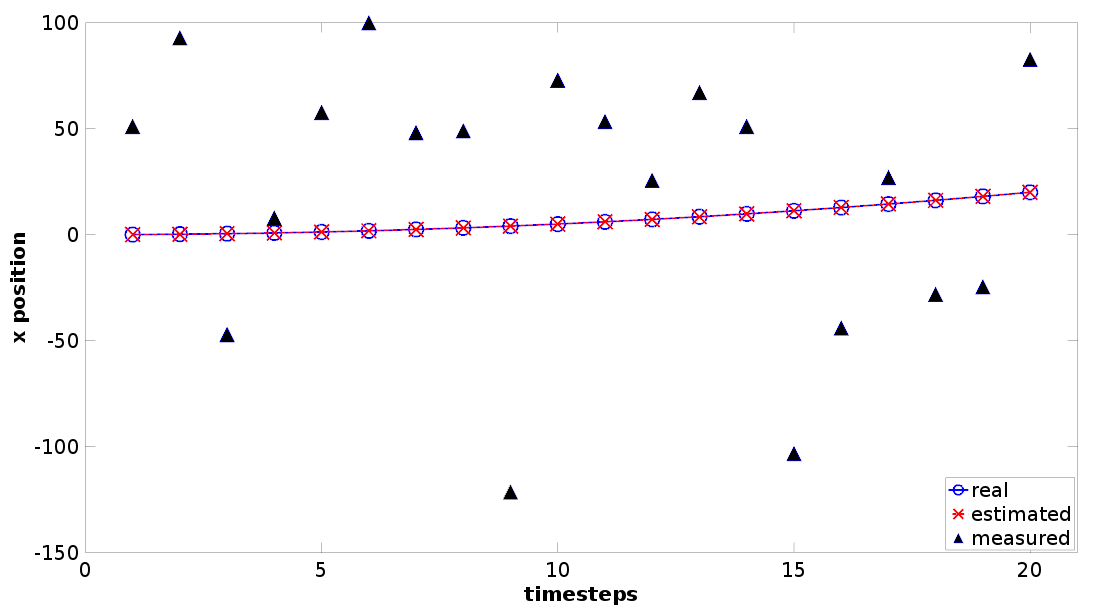
\includegraphics[width=\linewidth]{ps_a0m100}
	\captionof{figure}{Stima nelle prime 20 iterazioni ponendo $\sigma_{acc} = 0$ e $\sigma_{pos} = 100$ (partenza perfetta).} 
	\label{ps_a0m100} 
\end{minipage}

\begin{minipage}{\linewidth}
	\centering
	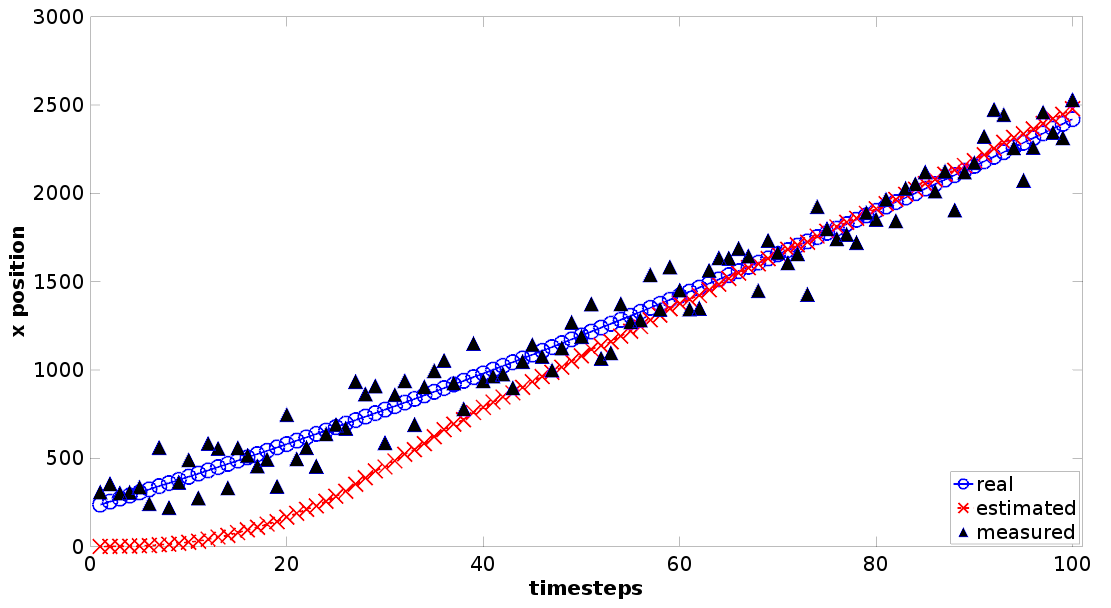
\includegraphics[width=\linewidth]{ws_a0m100_long}
	\captionof{figure}{Stima nelle prime 100 iterazioni ponendo $\sigma_{acc} = 0$ e $\sigma_{pos} = 100$ (partenza falsata).} 
	\label{ws_a0m100_long}
\end{minipage}

\end{itemize}

\section{Simulazione di un processo non lineare}

Il Kalman filter è interamente specificato tramite matrici; pertanto, esso si presta a modellare unicamente quei processi che presentano transizioni di stato lineari. Si può dimostrare che se la distribuzione di probabilità è una gaussiana multivariata e il modello di transizione è lineare, applicare l'operazione di filtering in un modello probabilistico temporale ha come risultato un'altra distribuzione gaussiana multivariata. Il modello di transizione lineare è quindi un'assunzione necessaria per garantire la convergenza del metodo. Per questo motivo il Kalman filter non è adatto a simulare processi non lineari, come dimostra il seguente esperimento.

Il processo che si vorrebbe simulare è l'evoluzione della coppia $\langle x, x^2 \rangle$ al variare di $x$. Nel caso in esame si assume che $x$ venga incrementata di una quantità costante $\dx > 0$ ad ogni iterazione. Pertanto, fissato $\dx$, idealmente lo stato corrente \textbf{x} e quello successivo \textbf{x'} sono rappresentati dai vettori:
\begin{equation*}
\textbf{x} = 
\begin{bmatrix}
x^2 \\
x \\
\end{bmatrix}
\qquad
\textbf{x'} = 
\begin{bmatrix}
(x + \dx)^2 \\
x + \dx \\
\end{bmatrix}
\end{equation*}
Poiché la transizione di stato deve essere espressa linearmente si è fatto ricorso alla formula di Taylor di ordine 1, applicata alla funzione $x^2$ (ponendo $a = 1$):
\begin{equation}
\label{eq_taylor}
f(x) \approx f(a) + f'(a)(x-a) \qquad \mapsto  \qquad x^2 \approx 1 + 2(x-1)
\end{equation}
La matrice di transizione di stato \textbf{A}, la matrice di control input \textbf{B} e il relativo vettore di control input \textbf{u} sono definiti di conseguenza come :
\begin{equation*}
\textbf{A} = 
\begin{bmatrix}
0 & 2 \\
0 & 1 \\
\end{bmatrix}
\qquad 
\textbf{B} = 
\begin{bmatrix}
1 & 0\\
0 & 1\\
\end{bmatrix}
\qquad 
\textbf{u} = 
\begin{bmatrix}
2\dx -1 \\
\dx \\
\end{bmatrix}
\end{equation*}
In questo modo, lo stato successivo predetto dal modello è:
\begin{equation*}
\mathbf{x}^{(p)}_{t+1} = \mathbf{A x + B u} = 
\begin{bmatrix}
2x + 2\dx -1 \\
x + \dx \\
\end{bmatrix}  = 
\begin{bmatrix}
1 + 2(x + \dx -1) \\
x + \dx \\
\end{bmatrix} 
\end{equation*}
in accordo con quanto previsto dall'equazione \ref{eq_taylor}.

Le matrici di covarianza del rumore di processo e del rumore di misurazione sono definite come:
\begin{equation*}
\textbf{Q} = 
\begin{bmatrix}
\sigma_{proc}^4 & \sigma_{proc}^3 \\
\sigma_{proc}^3  & \sigma_{proc}^2 \\
\end{bmatrix}
\qquad 
\textbf{R} = 
\begin{bmatrix}
\sigma_{meas}^2 \\
\end{bmatrix}
\end{equation*}
dove $\sigma_{proc}$ è la deviazione standard del rumore di processo che influenza la variabile $x$ e che segue una distribuzione gaussiana $\mathcal{N}(0; \sigma_{proc}^2)$, mentre $\sigma_{meas}$ è la deviazione standard del rumore di misurazione che segue una distribuzione gaussiana $\mathcal{N}(0; \sigma_{meas}^2)$.\\
Infine, per semplicità si è assunta una partenza perfetta ponendo $\mathbf{x_0 = x_{real}} = \begin{bmatrix} 0 & 0 \end{bmatrix}^T$ e $\mathbf{P_0 = 0}$.

I test sono stati condotti considerando due situazioni differenti: nella prima la variabile di stato osservata è $x^2$, nella seconda invece è $x$. In tutti i casi si è posto $\dx = 0.4$ e sono state effettuate 100 iterazioni; pertanto risulta $x \in [0,40]$ (ignorando il rumore di processo, che può allargare/restringere tale intervallo).
\begin{itemize}
\item \textbf{Osservazione di $x^2$}\\
Nel caso  in cui il rumore di processo risulti trascurabile rispetto al rumore di misurazione ($\sigma_{proc} = 0.01$ e $\sigma_{meas} = 1$) il Kalman filter fa maggiore affidamento al modello, e sfrutta poco le osservazioni per correggere le proprie previsioni. In figura \ref{ox2_p001m1} è possibile osservare come il modello di transizione lineare porti lo stimatore a commettere un errore sempre maggiore man mano che ci si allontana dal punto in cui la formula di Taylor è stata calcolata ($a = 1$).
Anche la stima di $x$ è completamente falsata dall'utilizzo di un modello di transizione lineare, il quale non è in grado di simulare il processo reale in modo accurato (figura \ref{ox2_p001m1_x}).

\begin{minipage}{\linewidth}
	\centering
	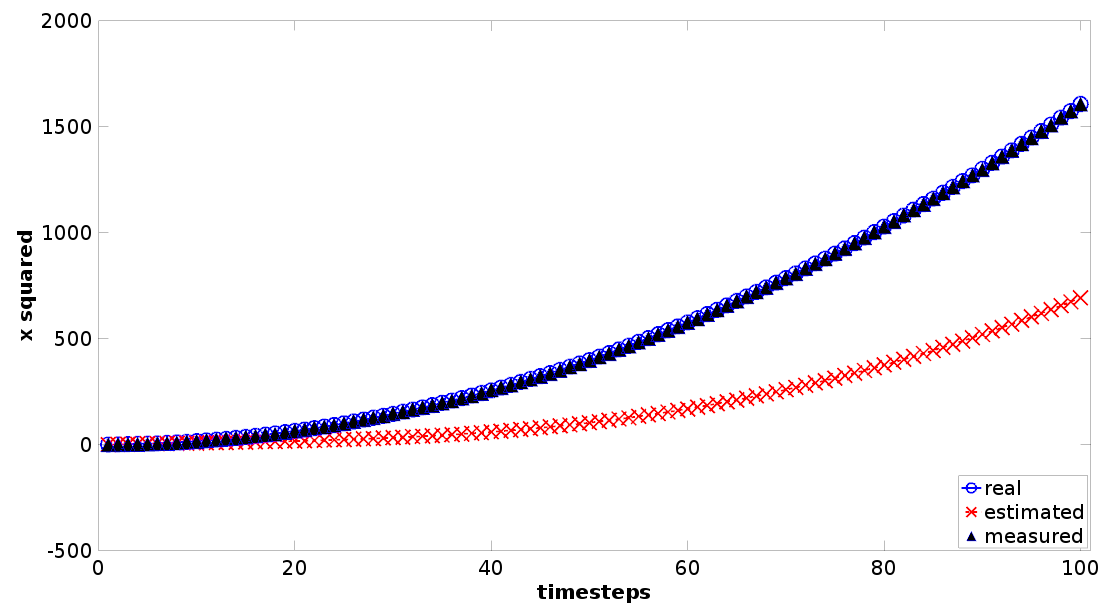
\includegraphics[width=\linewidth]{ox2_p001m1}
	\captionof{figure}{Stima di $x^2$ nelle prime 100 iterazioni, ponendo $\sigma_{proc} = 0.01$ e $\sigma_{meas} = 1$.} 
	\label{ox2_p001m1} 
\end{minipage}

\begin{minipage}{\linewidth}
	\centering
	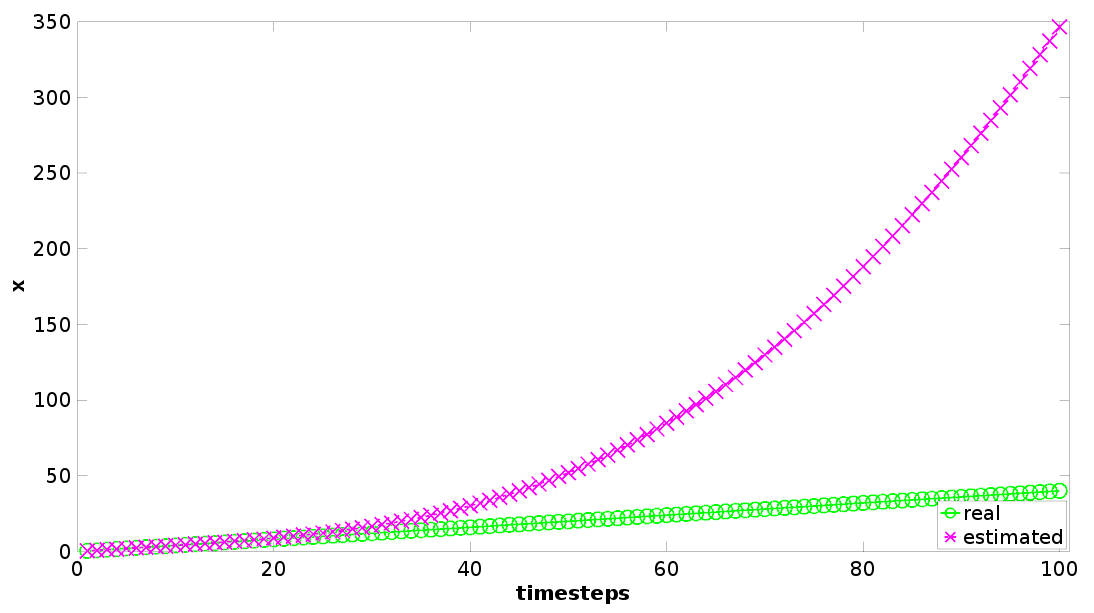
\includegraphics[width=\linewidth]{ox2_p001m1_x}
	\captionof{figure}{Stima di $x$ nelle prime 100 iterazioni, ponendo $\sigma_{proc} = 0.01$ e $\sigma_{meas} = 1$.} 
	\label{ox2_p001m1_x}
\end{minipage}

Al contrario, se il rumore di processo è alto rispetto al rumore di misurazione ($\sigma_{proc} = 1$ e $\sigma_{meas} = 0.01$), lo stimatore si affida alle osservazioni. In questo caso il Kalman filter approssima piuttosto bene il valore di $x^2$, ma il valore di $x$ risulta comunque estremamente inaccurato a causa del modello di transizione lineare: proprio quest'ultimo è infatti l'unico mezzo di cui il Kalman filter dispone per effettuare una stima di $x$.

\begin{minipage}{\linewidth}
	\centering
	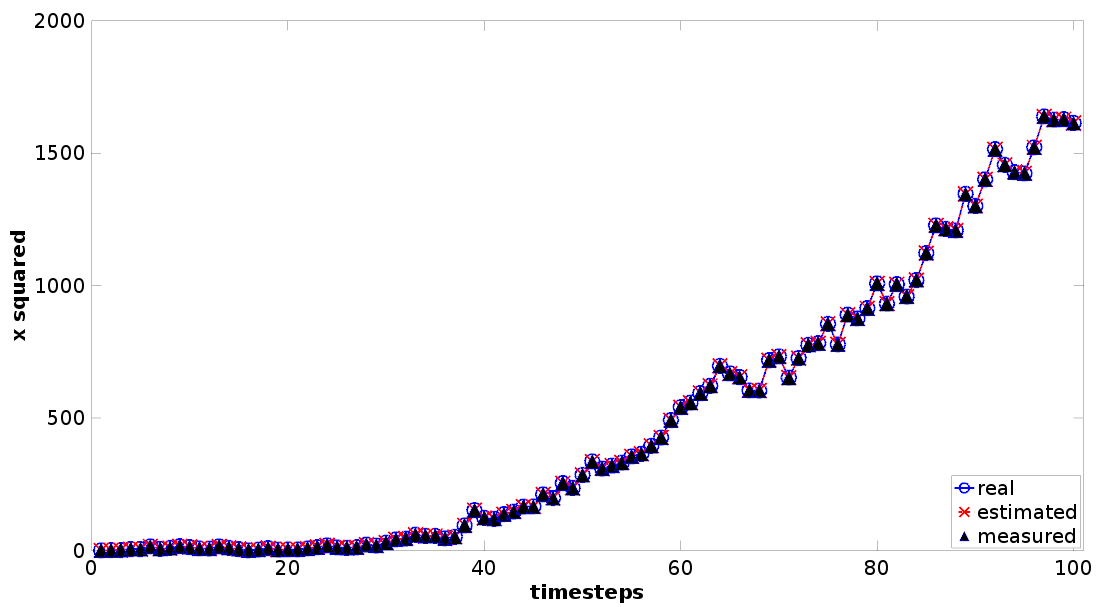
\includegraphics[width=\linewidth]{ox2_p1m001}
	\captionof{figure}{Stima di $x^2$ nelle prime 100 iterazioni, ponendo $\sigma_{proc} = 1$ e $\sigma_{meas} = 0.01$.} 
	\label{ps_a0m100} 
\end{minipage}

\begin{minipage}{\linewidth}
	\centering
	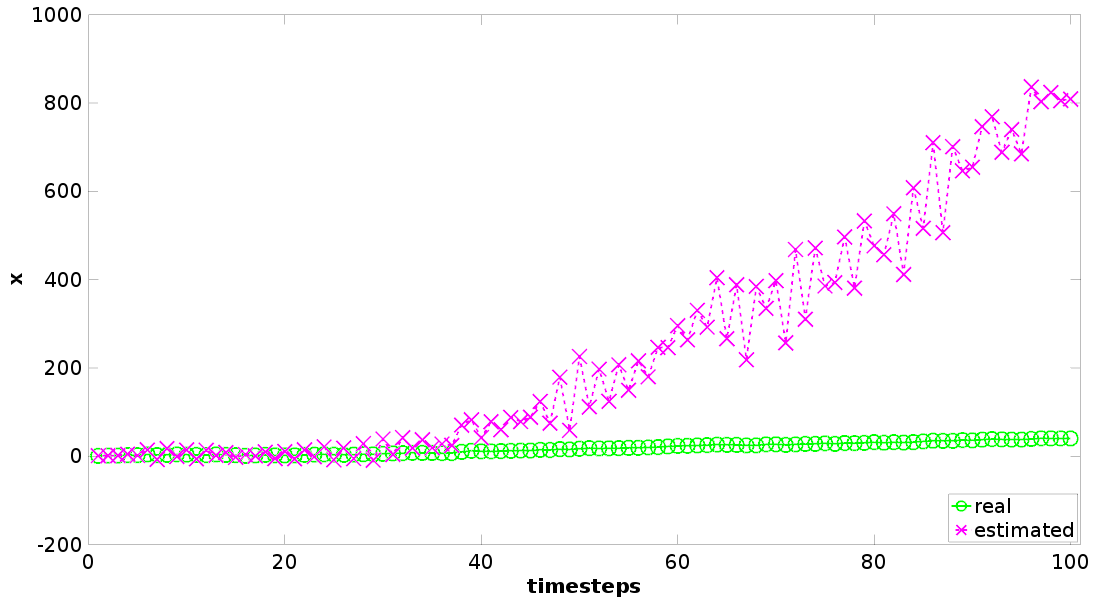
\includegraphics[width=\linewidth]{ox2_p1m001_x}
	\captionof{figure}{Stima di $x$ nelle prime 100 iterazioni, ponendo $\sigma_{proc} = 1$ e $\sigma_{meas} = 0.01$.} 
	\label{ws_a0m100_long}
\end{minipage}

\item \textbf{Osservazione di $x$}\\
Se la variabile di stato osservata non è $x^2$ bensì $x$, la situazione generale non migliora: il Kalman filter, potenzialmente, riesce ad approssimare bene $x$; nonostante ciò l'errore commesso nella stima di $x^2$ è destinato ad aumentare man mano che ci si allontana dal punto in cui è stata calcolata la formula di Taylor (dove l'approssimazione lineare della funzione quadratica risulta ottimale). 
\end{itemize}

In conclusione, il processo reale non può essere approssimato nella sua interezza a causa delle forti restrizioni imposte dal modello di transizione lineare. I risultati ottenuti suggeriscono tuttavia un possibile approccio per trattare anche processi non lineari: se si potesse calcolare ``dinamicamente" la formula di Taylor modificando il punto $a$ ad ogni iterazione, la simulazione del processo sarebbe decisamente migliore. Questa è l'idea che sta alla base del cosiddetto Extended Kalman Filter.













\end{document}

